\documentclass[11pt,a4paper]{article}

%
% Queries:
%  p. 1: What does "not C in general" in the solution of prelim 1 mean?
%  p. 5: $c + d = CH$ where $H$ is the intersection point of $c(C',d)$ and $c(D,e)$  on line $CC'$. Why does $H$ lie on line $CC'$?

%
% Typos
%  p. 2: cyclid quadrilateral -> cyclic quadrilateral
%  p. 4: \triangle AZB = \triangle BZK -> \triangle AZB = \triangle HZK
%  p. 5: Preliminary problem 3 -> Preliminary problem 4


\usepackage{mathpazo}
\usepackage{microtype}
\usepackage{url}
\usepackage{verbatim}

\usepackage{tikz}
\usetikzlibrary{external,positioning,through,calc,intersections}
\tikzexternalize[prefix=tikz/]


\textwidth=15cm
\textheight=23cm
\topmargin=1cm
\headheight=0pt
\oddsidemargin=2em
\headsep=0pt
\renewcommand{\baselinestretch}{1.1}
\setlength{\parskip}{0.5\baselineskip plus 1pt minus 1pt}
\parindent=0pt

\newcommand*{\qed}{%
$\quad\quad$\raisebox{2pt}{\framebox[10pt]{\rule{0pt}{4pt}}}%
}

\begin{document}

\textbf{\LARGE 33. Mascheroni's Compass Problem}

\begin{quote}
The construction presented in this document is taken from the book by Heinrich D\"{o}rrie: \textit{100 Problems of Elementary Mathematics: Their History and Solution} (Dover, 1965), as reworked by Michael Woltermann.\footnote{\url{http://www2.washjeff.edu/users/mwoltermann/Dorrie/DorrieContents.htm}.} The document is written in \LaTeX{} and I have redrawn the diagrams using Ti\textit{k}Z, often drawing a diagram incrementally for clarity. I have added explanations so that students and teachers can better understand the construction.

\begin{quote}
Moti Ben-Ari\footnote{\url{http://www.weizmann.ac.il/sci-tea/benari/}.}\\
Department of Science Teaching\\
Weizmann Institute of Science
\end{quote}
\end{quote}

%%%%%%%%%%%%%%%%%%%%%%%%%%%%%%%%%%%%%%%%%%%%%%%%%%%%%%%%%%%%%%%

Prove that any construction that can be carried out with a compass and straight-edge can be carried out with the compass alone. The Italian L. Mascheroni (1750-1800) posed this problem to himself and solved it in a masterly fashion in his book \textit{La geometria del compasso}, published in Pavia in 1797.

\begin{quote}
The theorem is known as the Mohr-Mascheroni Theorem since it had been proved in 1672 by the Danish mathematician Georg Mohr, but his work was not widely known until the twentieth century.
\end{quote}

When we examine the separate steps by which circle and straight-edge constructions are carried out, we see that every step consists of one of the following three basic constructions:

I. Finding the point of intersection of two straight lines;

II. finding the point of intersection of a straight line and a circle;

III. finding the point(s) of intersection of two circles.

Thus we need only show that the two basic constructions I. and II. can be done with a compass alone. (Mascheroni regarded a straight line as given if two of its points are known.)

First we will solve four preliminary problems. (Dörrie talks about two, but the others are embedded in these.) In the following:
\begin{itemize}
\item $C(O,A)$ stands for the circle with center $O$ through point $A$,
\item $C(O,AB)$ stands for the circle with center $O$ and radius $AB$.
\end{itemize}

%%%%%%%%%%%%%%%%%%%%%%%%%%%%%%%%%%%%%%%%%%%%%%%%%%%%%%%%%%%%%%%

\textbf{Prelim 1.} Reflect a point $C$ about the line through $A$ and $B$.

\begin{quote}
Given a point $C$ and a line $AB$, a reflection of $C$ about $AB$ is a point $C'$ such that $AB$ is the perpendicular bisector of the line $CC'$.
\end{quote}

\textbf{Solution.} The reflection $C'=c(A,C) \cap c(B,C)$ (not $C$ in general):

\begin{center}
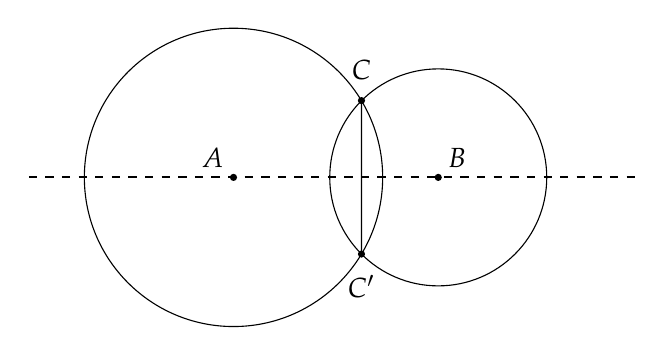
\begin{tikzpicture}[scale=.65]
\coordinate (A) at (0,0);
\coordinate (B) at (4,0);
\coordinate (C) at (2.5,1.5);
\draw[thick,dashed] ($(B)!2!(A)$) -- ($(A)!2!(B)$);
\fill (A) node[above left] {$A$} circle[radius=2pt];
\fill (B) node[above right] {$B$} circle[radius=2pt];
\fill (C) node[above,yshift=4pt] {$C$} circle[radius=2pt];
\node[draw,circle through=(C),name path=ac] at (A) {};
\node[draw,circle through=(C),name path=bc] at (B) {};
\path [name intersections={of=ac and bc,by={x1,Cp}}];
\fill (Cp) node[below,yshift=-4pt] {$C'$} circle[radius=2pt];
\draw (C) -- (Cp);
\end{tikzpicture}

{\centering Line $AB$ is the perpendicular bisector of chord $CC'$ of both circles}
\end{center}

Note: Dashed lines in figures are drawn to explain the arguments, but are not used in constructions.  \qed
\begin{quote}
This is important: the lines drawn in the diagrams serve only to illustrate the proofs; you must convince yourself that only a compass is used in all the constructions. I have added and modified lines, both solid and dashed, to clarify the diagrams.
\end{quote}

%%%%%%%%%%%%%%%%%%%%%%%%%%%%%%%%%%%%%%%%%%%%%%%%%%%%%%%%%%%%%%%

\textbf{Prelim 2.} Construct $c(A,BC)$, given points $A,B,C$.

\textbf{Solution.} Let $X$ and $Y$ be the points of intersection of $c(A,B)$ and $c(B,A)$:

\begin{center}
\begin{tikzpicture}[scale=.6]
\coordinate (A) at (0,1.5);
\coordinate (B) at (0,-1.5);
\coordinate (C) at (1.5,-3);
\coordinate (Cp) at (1.5,3);
\fill (A) node[above] {$A$} circle[radius=2pt];
\fill (B) node[below] {$B$} circle[radius=2pt];
\fill (C) node[below] {$C$} circle[radius=2pt];
\node[draw,circle through=(B),name path=ab] at (A) {};
\node[draw,circle through=(A),name path=ba] at (B) {};
\path [name intersections={of=ab and ba,by={Y,X}}];
\fill (X) node[above right,xshift=4pt] {$X$} circle[radius=2pt];
\fill (Y) node[above left,xshift=-4pt] {$Y$} circle[radius=2pt];
\draw[thick,dashed] ($(X)!2.3!(Y)$) -- ($(Y)!2!(X)$);
\end{tikzpicture}
\end{center}

Let $C'$ be the reflection of $C$ about line $XY$:

\begin{center}
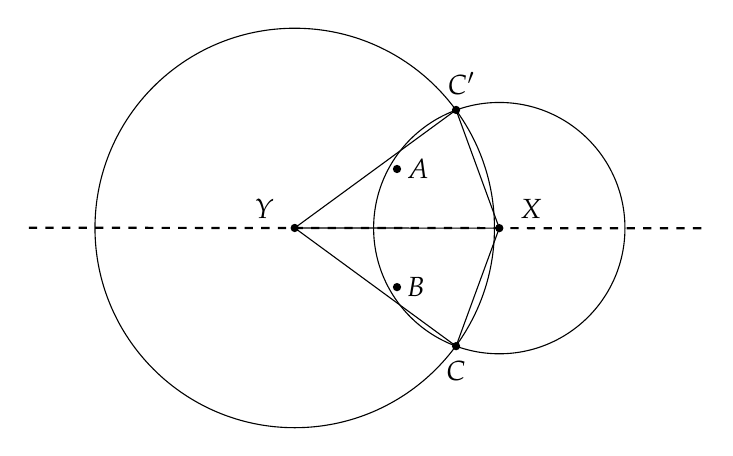
\begin{tikzpicture}[scale=.5]
\coordinate (A) at (0,1.5);
\coordinate (B) at (0,-1.5);
\coordinate (C) at (1.5,-3);
\coordinate (Cp) at (1.5,3);
\fill (A) node[right] {$A$} circle[radius=3pt];
\fill (B) node[right] {$B$} circle[radius=3pt];
\fill (C) node[below,yshift=-2pt] {$C$} circle[radius=3pt];
\fill (Cp) node[above,xshift=2pt,yshift=2pt] {$C'$} circle[radius=3pt];
\node[circle through=(B),name path=ab] at (A) {};
\node[circle through=(A),name path=ba] at (B) {};
\path [name intersections={of=ab and ba,by={Y,X}}];
\fill (X) node[above right,xshift=4pt] {$X$} circle[radius=3pt];
\fill (Y) node[above left,xshift=-4pt] {$Y$} circle[radius=3pt];
\node[draw,circle through=(C)] at (X) {};
\node[draw,circle through=(C)] at (Y) {};
\draw[thick,dashed] ($(X)!2.3!(Y)$) -- ($(Y)!2!(X)$);
\draw (X) -- (Y) -- (C) -- (X) -- (Cp) -- (Y);
\end{tikzpicture}
\end{center}

\begin{quote}
Since $XC=XC', YC=YC', XY=XY$, the triangles $\triangle XYC, XYC'$ are congruent; therefore, the length of the altitude from $C$ to $XY$ equals the length of the altitude from $C'$ to $XY$. It follows that $XY$ is the perpendicular bisector of $CC'$, so $C'$ is the reflection of $C$ about $XY$.
\end{quote}

$c(A,C')$ is the desired circle:

\begin{center}
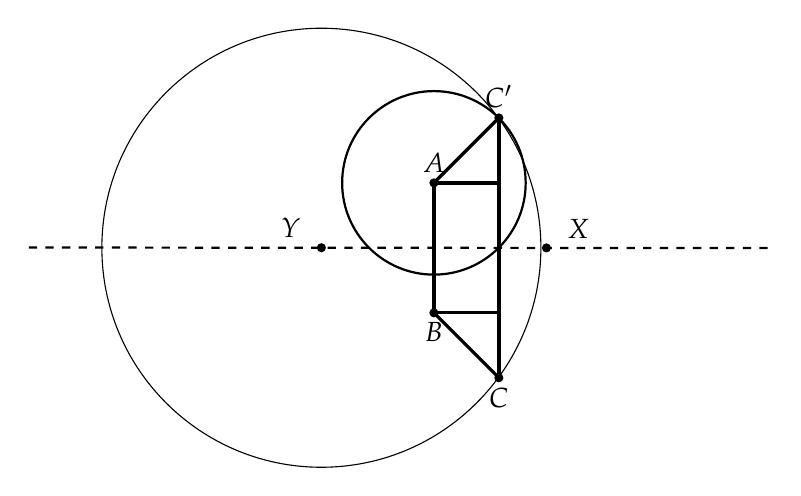
\begin{tikzpicture}[scale=.55]
\coordinate (A) at (0,1.5);
\coordinate (B) at (0,-1.5);
\coordinate (C) at (1.5,-3);
\coordinate (Cp) at (1.5,3);
\fill (A) node[above] {$A$} circle[radius=3pt];
\fill (B) node[below] {$B$} circle[radius=3pt];
\fill (C) node[below] {$C$} circle[radius=3pt];
\fill (Cp) node[above] {$C'$} circle[radius=3pt];
\node[circle through=(B),name path=ab] at (A) {};
\node[circle through=(A),name path=ba] at (B) {};
\path [name intersections={of=ab and ba,by={Y,X}}];
\fill (X) node[above right,xshift=4pt] {$X$} circle[radius=3pt];
\fill (Y) node[above left,xshift=-4pt] {$Y$} circle[radius=3pt];
\node[circle through=(C)] at (X) {};
\node[draw,circle through=(C)] at (Y) {};
\draw[thick,dashed] ($(X)!2.3!(Y)$) -- ($(Y)!2!(X)$);
\node[draw,thick,circle through=(Cp)] at (A) {};
\draw[very thick] (A) -- (Cp);
\draw[very thick] (B) -- (C);
\draw[very thick] (A) -- (B);
\draw[very thick] (C) -- (Cp);
\draw[very thick] (A) -| (C);
\draw[very thick] (B) -| (C);
\end{tikzpicture}
\end{center}

(Since $A$ is the reflection of $B$ about $XY$, and reflection preserves distance, so $AC'=BC$.) \qed

\begin{quote}
Reasoning similar to that above that $C'$ is a reflection of $C$ shows that $A$ is the reflection of $B$ about $XY$. The thick lines show how $AC'=BC$ can be proved using congruent triangles.

In general, it is a theorem that reflection  preserves distance. This is proved in high-school textbooks, such as Theorem~6.1 of Ann Xavier Gantert, \textit{Geometry} (AMSCO, 2008).
\end{quote}

%%%%%%%%%%%%%%%%%%%%%%%%%%%%%%%%%%%%%%%%%%%%%%%%%%%%%%%%%%%%%%%

\textbf{Prelim 3.} Construct the sum or difference of two given segments $a$ and $b$, i.e., lengthen or shorten a given segment $PQ = a$ by a segment $QX = b$. (See Prelim 2 if necessary to construct a segment of length $b$ at $Q$.)

\textbf{Solution.}

1. Let $H$ be any point on $c(Q,b)$, and $H'$ its reflection about line $PQ$. Let $h$ be the (length of) segment $HH'$:

\begin{center}
\begin{tikzpicture}[scale=.6]
\coordinate (Q) at (0,0);
\coordinate (P) at (-6.8,0);
\coordinate (B) at (-3,-2);
\draw[thick,dashed] ($(Q)!1.3!(P)$) -- ($(P)!2.3!(Q)$);
\fill (Q) node[above left] {$Q$} circle[radius=2pt];
\fill (P) node[above] {$P$} circle[radius=2pt];
\fill (B) circle[radius=2pt];
\node[draw,circle through=(B),name path=qb] at (Q) {};
\draw[thick,dashed] (Q) -- node[left,xshift=-1pt,yshift=2pt] {$b$} (B);
\path[name path=qh] (Q) -- (-40:5cm);
\path[name path=qhp] (Q) -- (40:5cm);
\path [name intersections={of=qb and qh,by={H}}];
\path [name intersections={of=qb and qhp,by={Hp}}];
\fill[below right] (H) node[right,xshift=2pt] {$H$} circle[radius=2pt];
\fill[above right] (Hp) node[right,xshift=2pt] {$H'$} circle[radius=2pt];
\draw[thick,dashed] (H) -- node[below left,yshift=-2pt] {$h$} (Hp);
\end{tikzpicture}
\end{center}

2. Let $K = c(Q,h) \cap c(H,b)$:

\begin{center}
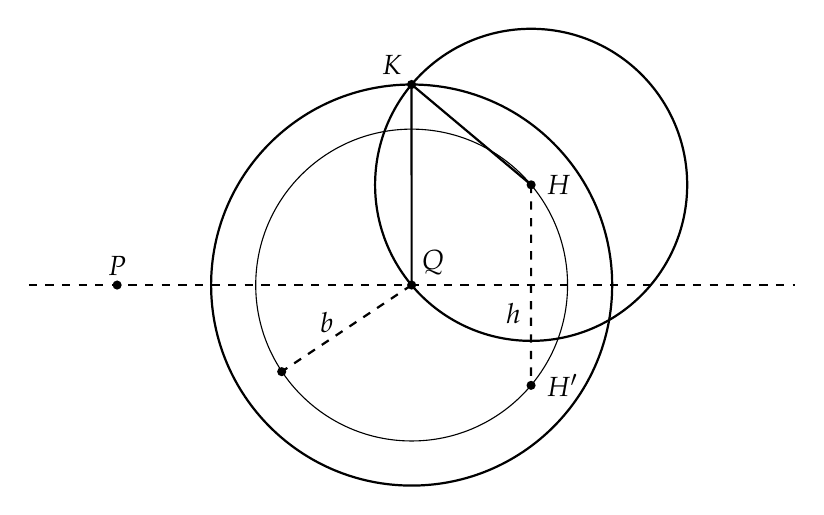
\begin{tikzpicture}[scale=.55]
\coordinate (Q) at (0,0);
\coordinate (P) at (-6.8,0);
\coordinate (B) at (-3,-2);
\draw[thick,dashed] ($(Q)!1.3!(P)$) -- ($(P)!2.3!(Q)$);
\fill (Q) node[above right] {$Q$} circle[radius=3pt];
\fill (P) node[above] {$P$} circle[radius=3pt];
\fill (B) circle[radius=3pt];
\node[draw,circle through=(B),name path=qb] at (Q) {};
\draw[thick,dashed] (Q) -- node[left,xshift=-1pt,yshift=2pt] {$b$} (B);
\path[name path=qh] (Q) -- (-40:5cm);
\path[name path=qhp] (Q) -- (40:5cm);
\path [name intersections={of=qb and qh,by={Hp}}];
\path [name intersections={of=qb and qhp,by={H}}];
\fill (H) node[right,xshift=2pt] {$H$} circle[radius=3pt];
\fill (Hp) node[right,xshift=2pt] {$H'$} circle[radius=3pt];
\draw[thick,dashed] (H) -- node[below left,yshift=-3pt] {$h$} (Hp);
\draw[thick,name path=circleqh] (Q) let
  \p1 = ($ (H) - (Hp) $)
in
  circle ({veclen(\x1,\y1)});
\draw[thick,name path=circlehb] (H) let
  \p1 = ($ (Q) - (B) $)
in
  circle ({veclen(\x1,\y1)});
\path [name intersections={of=circleqh and circlehb,by={K,k2}}];
\fill (K) node[above left] {$K$} circle[radius=3pt];
\draw[thick] (Q) -- (K);
\draw[thick] (H) -- (K);
\end{tikzpicture}
\end{center}

and $K'$ be the reflection of $K$ about line $PQ$.

Then $KHH'K'$ is an isosceles trapezoid with legs $KH = K'H' = b$ and base $KK' = 2h$. Let $d = KH' = K'H$:

\begin{quote}
$H'$ is a reflection of $H$ and $K'$ is a reflection of $K$. Since reflections preserve distance, $KH=K'H'$.
\end{quote}

\begin{center}
\begin{tikzpicture}[scale=.6]
\coordinate (Q) at (0,0);
\coordinate (P) at (-6.8,0);
\coordinate (B) at (-3,-2);
\draw[thick,dashed] ($(Q)!1.3!(P)$) -- ($(P)!2.3!(Q)$);
\fill (Q) node[above left] {$Q$} circle[radius=3pt];
\fill (P) node[above] {$P$} circle[radius=3pt];
\fill (B) circle[radius=3pt];
\node[draw,circle through=(B),name path=qb] at (Q) {};
\draw[thick,dashed] (Q) -- node[left,xshift=-1pt,yshift=2pt] {$b$} (B);
\path[name path=qh] (Q) -- (-40:5cm);
\path[name path=qhp] (Q) -- (40:5cm);
\path [name intersections={of=qb and qh,by={Hp}}];
\path [name intersections={of=qb and qhp,by={H}}];
\fill (H) node[right,xshift=2pt] {$H$} circle[radius=3pt];
\fill (Hp) node[right,xshift=2pt] {$H'$} circle[radius=3pt];
\draw (H) -- node[below right,yshift=-2pt] {$h$} (Hp);
\path[name path=circleqh] (Q) let
  \p1 = ($ (H) - (Hp) $)
in
  circle ({veclen(\x1,\y1)});
\path[name path=circlehb] (H) let
  \p1 = ($ (Q) - (B) $)
in
  circle ({veclen(\x1,\y1)});
\path [name intersections={of=circleqh and circlehb,by={K,k2}}];
\fill (K) node[above left] {$K$} circle[radius=3pt];
\draw (Q) -- node[left] {$h$} (K);
\draw (H) -- node[right,xshift=2pt] {$b$} (K);
\draw let
  \p1 = ($ (K) - (Q) $)
in
  coordinate (Kp) at (\x1,-\y1);
\fill (Kp) node[below left] {$K'$} circle[radius=3pt];
\draw (Q) -- node[left] {$h$} (Kp) -- node[right,xshift=2pt] {$b$} (Hp);
\draw (K) -- node[above right] {$d$} (Hp);
\draw (Kp) -- node[left] {$d$} (H);
\end{tikzpicture}
\label{ptolemy}
\end{center}


Since opposite angles of $KHH'K'$ are supplemental, $KHH'K'$ is a cyclic quadrilateral, i.e., it can be inscribed in a circle. 

\begin{quote}
Geometry textbooks give the simple proof that the opposite angles of a cyclic quadrilateral are supplementary (add up to $180^\circ$), but it is hard to find a proof of the converse, so I present the proofs here:

\begin{center}
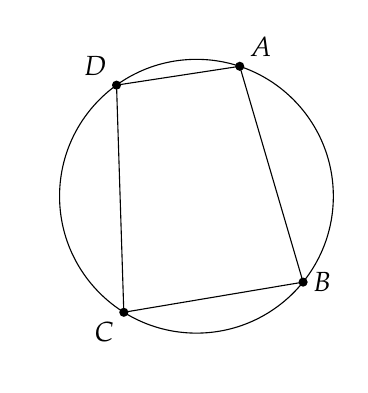
\begin{tikzpicture}[scale=.55]
\coordinate (origin) at (0,0);
\coordinate (A) at (1,3);
\node[draw,circle through=(A),name path=circle] at (origin) {};
\fill (A) node[above right] {$A$} circle[radius=3pt];
\path[name path=b] (A) -- (-50:4.5cm);
\path[name path=c] (A) -- (-120:4.5cm);
\path[name path=d] (A) -- (150:4.5cm);
\path [name intersections={of=circle and b,by={b1,B}}];
\fill (B) node[right] {$B$} circle[radius=3pt];
\path [name intersections={of=circle and c,by={c1,C}}];
\fill (C) node[below left] {$C$} circle[radius=3pt];
\path [name intersections={of=circle and d,by={d1,D}}];
\fill (D) node[above left] {$D$} circle[radius=3pt];
\draw (A) -- (B) -- (C) -- (D) -- cycle;
\end{tikzpicture}
\end{center}

Proof that the opposite angles of a cyclic quadilateral are supplementary: Recall that an inscribed angle equals half the subtended arc. So $\angle DAB$ is half of the arc $DCB$ and $\angle DCB$ is half of the arc $DAB$. But the two arcs form the entire circumference of the circle so their sum is $360^\circ$ and $\angle DAB + \angle DCB = \frac{1}{2} \cdot 360^\circ =  180^\circ$.

Proof that a quadilateral whose opposite sides are supplementary is cyclic: Any triangle can be inscribed in a circle. Suppose that the triangle $\triangle DAB$ is inscribed in the circle and suppose that $C'$ is a point such that $\angle DAB + \angle DC'B = 180^\circ$ but $C'$ is \emph{not} on the circumference of the circle. Without loss of generality, let $C'$ be within the circle:

\begin{center}
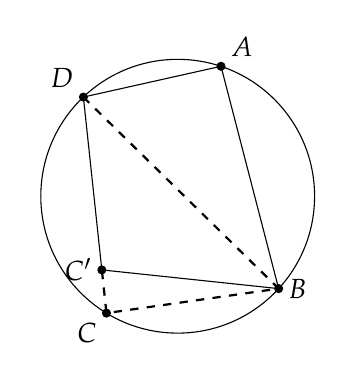
\begin{tikzpicture}[scale=.55]
\coordinate (origin) at (0,0);
\coordinate (A) at (1,3);
\node[draw,circle through=(A),name path=circle] at (origin) {};
\fill (A) node[above right] {$A$} circle[radius=3pt];
\path[name path=b] (A) -- (-50:4cm);
\path[name path=c] (A) -- (-120:4cm);
\path[name path=d] (A) -- (150:4cm);
\path [name intersections={of=circle and b,by={b1,B}}];
\fill (B) node[right] {$B$} circle[radius=3pt];
\path [name intersections={of=circle and c,by={c1,C}}];
\fill (C) node[below left] {$C$} circle[radius=3pt];
\path [name intersections={of=circle and d,by={d2,D}}];
\fill (D) node[above left] {$D$} circle[radius=3pt];
\coordinate (Cp) at ($(C)!.2!(D)$);
\draw (A) -- (B) -- (Cp) -- (D) -- cycle;
\fill (Cp) node[left] {$C'$} circle[radius=3pt];
\draw[thick,dashed] (D) -- (B) -- (C) -- (Cp);
\end{tikzpicture}
\end{center}

Construct a ray that extends $DC'$ and let $C$ be its intersection with the circle. By the forward direction of the theorem:
\begin{eqnarray*}
\angle DAB + \angle DCB &=& 180^\circ = \angle DAB + \angle DC'B\\
\angle DCB &=& \angle DC'B\,,
\end{eqnarray*}
which is impossible if $C$ and $C'$ are distinct points.

Let us complete the proof by showing that the opposite angles of an isosceles trapezoid are supplementary and therefore that an isosceles trapezoid is cycle:

\begin{center}
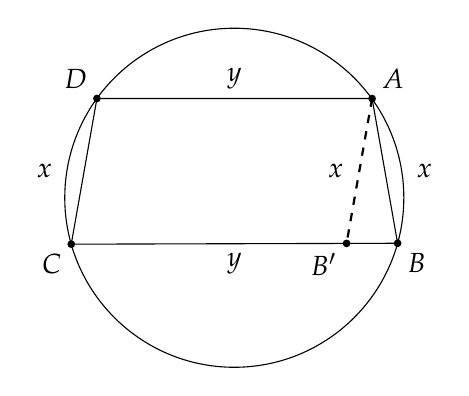
\begin{tikzpicture}[scale=.7]
\coordinate (origin) at (0,0);
\coordinate (A) at (2.5,1.8);
\node[draw,circle through=(A),name path=circle] at (origin) {};
\fill (A) node[above right] {$A$} circle[radius=2pt];
\path[name path=b] (A) -- ++(-80:4cm);
\path[name path=d] (A) -- ++(180:6cm);
\path [name intersections={of=circle and b,by={b1,B}}];
\fill (B) node[below right] {$B$} circle[radius=2pt];
\path [name intersections={of=circle and d,by={d1,D}}];
\fill (D) node[above left] {$D$} circle[radius=2pt];
\path[name path=c] (D) -- ++(-100:4cm);
\path [name intersections={of=circle and c,by={c1,C}}];
\fill (C) node[below left] {$C$} circle[radius=2pt];
\draw (A) -- node[right,xshift=8pt] {$x$} (B);
\draw[name path=bc] (B) -- node[below] {$y$} (C);
\draw (C) -- node[left,xshift=-8pt] {$x$} (D) -- node[above] {$y$} (A);
\path[name path=para] (A) -- ++(-100:4cm);
\path [name intersections={of=para and bc,by={Bp}}];
\fill (Bp) node[below left] {$B'$} circle[radius=2pt];
\draw[thick,dashed] (A) -- node[left,xshift=-2pt] {$x$} (Bp);
\end{tikzpicture}
\end{center}

Construct the line $AB'$ parallel to $CD$. Then $AB'CD$ is a parallelogram and $\triangle ABB'$ is an isosceles triangle. Therefore, $\angle C= \angle AB'B = \angle B$. A similar proof shows that $\angle A = \angle D$. Since the sum of the internal angles of any quadrilateral is equal to $360^\circ$:
\begin{eqnarray*}
\angle A + \angle B + \angle C + \angle D &=& 360^\circ\\
2\angle A + 2 \angle C &=& 360^\circ\\
\angle A +  \angle C &=& 180^\circ\,,
\end{eqnarray*}
and similarly, $\angle B +  \angle D = 180^\circ$.
\end{quote}

Then by Ptolemy’s theorem $d^2 = b^2 + 2h^2$.
\begin{quote}
Ptolemy's theorem states that for a quadrilateral inscribed in a circle, the following equality relates the lengths of the sides $a,b,c,d$ and the lengths of the diagonals $e,f$:
\[
ef = ac + bd\,.
\]
\begin{center}
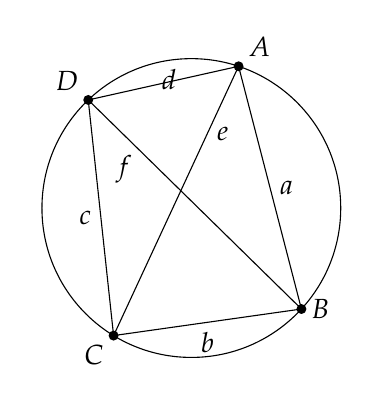
\begin{tikzpicture}[scale=.6]
\coordinate (origin) at (0,0);
\coordinate (A) at (1,3);
\node[draw,circle through=(A),name path=circle] at (origin) {};
\fill (A) node[above right] {$A$} circle[radius=3pt];
\path[name path=b] (A) -- (-50:4cm);
\path[name path=c] (A) -- (-120:4cm);
\path[name path=d] (A) -- (150:4cm);
\path [name intersections={of=circle and b,by={b1,B}}];
\fill (B) node[right] {$B$} circle[radius=3pt];
\path [name intersections={of=circle and c,by={C,c2}}];
\fill (C) node[below left] {$C$} circle[radius=3pt];
\path [name intersections={of=circle and d,by={D,d2}}];
\fill (D) node[above left] {$D$} circle[radius=3pt];
\draw (A) -- node[right] {$a$} (B) -- node[below] {$b$} (C) -- node[left] {$c$} (D) -- node[above,xshift=2pt,yshift=-6pt] {$d$}  cycle;
\draw (A) -- node[right,near start] {$e$} (C);
\draw (B) -- node[left,near end,yshift=-6pt] {$f$} (D);
\end{tikzpicture}
\end{center}
There is a geometric proof of the theorem (see Wikipedia), but I prefer to present a simple trigonometric proof. The law of cosines for the four triangles $\triangle ABC, \triangle ADC, \triangle DAB, \triangle DCB$ gives the following four equations:
\begin{eqnarray*}
e^2 &=& a^2 + b^2 - 2ab \cos \angle B\\
e^2 &=& c^2 + d^2 - 2cd \cos \angle D\\
f^2 &=& a^2 + d^2 - 2ad \cos \angle A\\
f^2 &=& b^2 + c^2 - 2bc \cos \angle C\,.
\end{eqnarray*}
The opposite angles of an inscribed quadrilateral are supplementary $\angle C = 180^\circ - \angle A$ and $\angle D = 180^\circ - \angle B$, so $\cos \angle D = - \cos \angle B$ and $\cos \angle C = -\cos \angle A$, and we can eliminate the cosines from the first two equations and from the last two equations. After some messy arithmetic, we get:
\begin{eqnarray*}
e^2 &=& \frac{(ac+bd)(ad+bc)}{(ab+cd)}\\
f^2 &=& \frac{(ab+cd)(ac+bd)}{(ad+bc)}\,.
\end{eqnarray*}
Multiply the two equations and simplify to get Ptolemy's theorem:
\begin{eqnarray*}
e^2\cdot f^2 &=& (ac+bd)^2\\
ef &=& (ac+bd)\,. 
\end{eqnarray*}
For the construction on page~\pageref{ptolemy}, the diagonals are of length $d$, the legs are of length $b$ and the parallel lines are of lengths $h$ and $2h$, so Ptolemy's theorem gives $d\cdot d = b\cdot b + h\cdot 2h$ or $d^2=b^2+2h^2$.
\end{quote}

Let $X$ be the point on line $PQ$ that extends $PQ$ by $b$. (We will eventually construct $X$; now we're just imagining it.)

Let $x = K'X$. Since $\triangle QK'X$ is a right triangle, $x^2 = b^2 + h^2$:
\begin{center}
\begin{tikzpicture}[scale=.7]
\coordinate (Q) at (0,0);
\coordinate (P) at (-6.8,0);
\coordinate (B) at (-3,-2);
\draw[thick,dashed,name path=pq] ($(Q)!1.3!(P)$) -- ($(P)!2.3!(Q)$);
\fill (Q) node[above left] {$Q$} circle[radius=2pt];
\fill (P) node[above] {$P$} circle[radius=2pt];
\fill (B) circle[radius=2pt];
\node[draw,circle through=(B),name path=qb] at (Q) {};
\draw[thick,dashed] (Q) -- node[left,xshift=-1pt,yshift=2pt] {$b$} (B);
\path[name path=qh] (Q) -- (-40:5cm);
\path[name path=qhp] (Q) -- (40:5cm);
\path [name intersections={of=qb and qh,by={hp}}];
\path [name intersections={of=qb and qhp,by={H}}];
\fill (H) node[right,xshift=2pt] {$H$} circle[radius=2pt];
\fill (hp) node[right,xshift=2pt] {$H'$} circle[radius=2pt];
\draw[thick,dashed] (H) -- (hp);
\path[name path=circleqh] (Q) let
  \p1 = ($ (H) - (hp) $)
in
  circle ({veclen(\x1,\y1)});
\path[name path=circlehb] (H) let
  \p1 = ($ (Q) - (B) $)
in
  circle ({veclen(\x1,\y1)});
\path [name intersections={of=circleqh and circlehb,by={K,k2}}];
\fill (K) node[above left] {$K$} circle[radius=2pt];
\draw[thick,dashed] (Q) -- (K);
\draw[thick,dashed] (H) -- (K);
\draw[thick,dashed] let
  \p1 = ($ (K) - (Q) $)
in
  coordinate (kp) at (\x1,-\y1);
\fill (kp) node[below left] {$K'$} circle[radius=2pt];
\draw[thick,dashed] (Q) -- node[left] {$h$} (kp) -- (hp);
\draw[thick,dashed] (K) -- (hp);
\draw[thick,dashed] (kp) -- (H);
\path [name intersections={of=pq and qb,by={X,x2}}];
\fill (X) node[below right] {$X$} circle[radius=2pt];
\draw[thick,dashed] (kp) -- node[left] {$x$} (X);
\draw[very thick] (Q) -- (kp) -- (X) -- node[above,xshift=-8pt] {$b$} cycle;
\end{tikzpicture}
\end{center}
It follows then that $d^2 = x^2 + h^2$ so that $x$ is a leg of a right triangle with hypotenuse $d$, the other leg being $h$.

\begin{quote}
By Ptolemy's theorem, $d^2 = b^2 + 2h^2$, so $d^2=(x^2-h^2)+2h^2=x^2+h^2$. All the previous sentence is saying is that it is possible to build a right triangle with sides $x,h,d$; such a triangle does not appear in the above diagram.
\end{quote}
Now let $S = c(K,d) \cap c(K',d)$.

$QS^2 + h^2 = d^2$, so $QS = x$:

\begin{center}
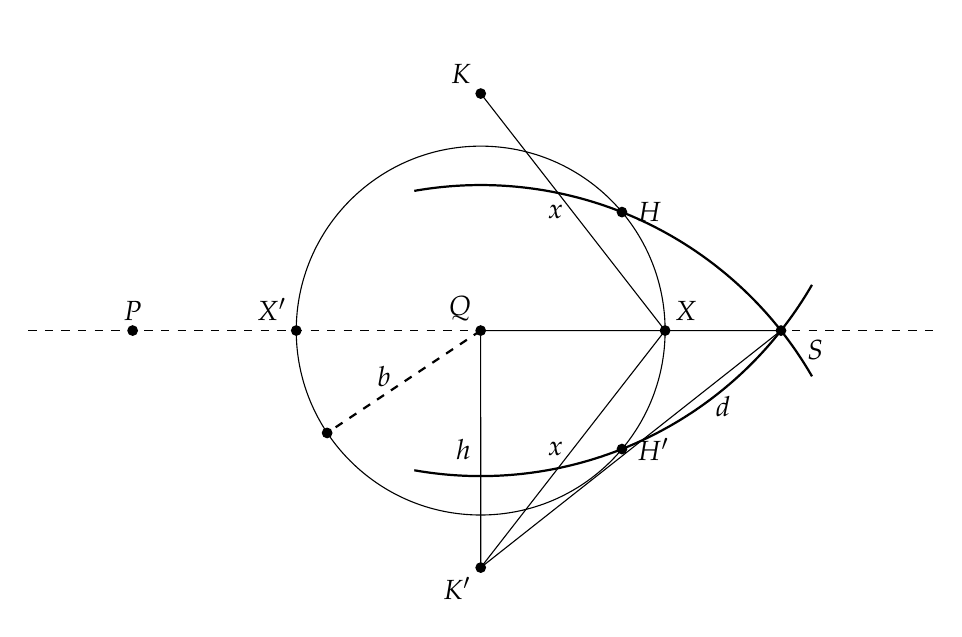
\begin{tikzpicture}[scale=.65]
\coordinate (Q) at (0,0);
\coordinate (P) at (-6.8,0);
\coordinate (B) at (-3,-2);
\draw[dashed,name path=pq] ($(Q)!1.3!(P)$) -- ($(P)!2.3!(Q)$);
\fill (Q) node[above left] {$Q$} circle[radius=3pt];
\fill (P) node[above] {$P$} circle[radius=3pt];
\node[draw,circle through=(B),name path=qb] at (Q) {};
\path[name path=qh] (Q) -- (-40:5cm);
\path[name path=qhp] (Q) -- (40:5cm);
\path [name intersections={of=qb and qh,by={Hp}}];
\path [name intersections={of=qb and qhp,by={H}}];
\fill (H) node[right,xshift=2pt] {$H$} circle[radius=3pt];
\fill (Hp) node[right,xshift=2pt] {$H'$} circle[radius=3pt];
\path[name path=circleqh] (Q) let
  \p1 = ($ (H) - (Hp) $)
in
  circle ({veclen(\x1,\y1)});
\path[name path=circlehb] (H) let
  \p1 = ($ (Q) - (B) $)
in
  circle ({veclen(\x1,\y1)});
\path [name intersections={of=circleqh and circlehb,by={K,k2}}];
\fill (K) node[above left] {$K$} circle[radius=3pt];
\draw[thick,dashed] let
  \p1 = ($ (K) - (Q) $)
in
  coordinate (Kp) at (\x1,-\y1);
\fill (Kp) node[below left] {$K'$} circle[radius=3pt];
\draw (Q) -- node[left] {$h$} (Kp);
\draw[thick,name path=khp] (K) let
  \p1 = ($ (H) - (Kp) $),
  \n2 = {veclen(\x1,\y1)}
in
  (K) ++(-100:\n2) arc (-100:-30:\n2);
\draw[thick,name path=kph] (Kp) let
  \p1 = ($ (H) - (Kp) $),
  \n2 = {veclen(\x1,\y1)}
in
  (Kp) ++(100:\n2) arc (100:30:\n2);
\path [name intersections={of=kph and khp,by={S}}];
\fill (S) node[below right,xshift=6pt] {$S$} circle[radius=3pt];
\draw (Kp) -- node[right,near end,yshift=-6pt] {$d$} (S);
\draw (Q) -- (S);
\path [name intersections={of=pq and qb,by={X,Xp}}];
\fill (X) node[above right] {$X$} circle[radius=3pt];
\fill (Xp) node[above left] {$X'$} circle[radius=3pt];
\draw (Kp) -- node[left] {$x$} (X);
\draw (K) -- node[left] {$x$} (X);
\fill (B) circle[radius=3pt];
\draw[thick,dashed] (Q) -- node[left,xshift=-1pt,yshift=2pt] {$b$} (B);
\end{tikzpicture}
\end{center}

3. Then $X = c(K,x) \cap c(K',x)$.

There are two $X$s, one for $a + b$ and one for $a - b$. \qed

\begin{quote}
Recall what we are trying to construct: extend $PQ$ of length $a$ by a length $b$. Since the length of $QX$ is $b$, the length of $PX$ is $a+b$. Similarly, the length of $PX'$ is $a-b$.
\end{quote}


%%%%%%%%%%%%%%%%%%%%%%%%%%%%%%%%%%%%%%%%%%%%%%%%%%%%%%%%%%%%%%%

\textbf{Prelim 4.} Given segments of length $n,m,s$, construct a segment of length $x = \frac{n}{m}s$.

\textbf{Solution.} This solution by Mascheroni is remarkable for its brevity and simplicity. Draw two concentric circles $c_1 = c(Z,m)$ and $c_2 = c(Z,n)$ and chord $AB = s$ on $c_1$. (It is assumed that $s$ falls within $c_1$. If not, use Prelim 3 to replace $n$ and $m$ by sufficiently large integer multiples $kn = N$ and $km = M$.)

\begin{quote}
There is an implicit assumption that $m>n$. If not, just exchange the notation.

The expression "it is assumed that $s$ falls within $c_1$" refers to the possibility that $s$ is within $c_1$ but also cuts through $c_2$. By using multiples this can be avoided.
\end{quote}

\begin{center}
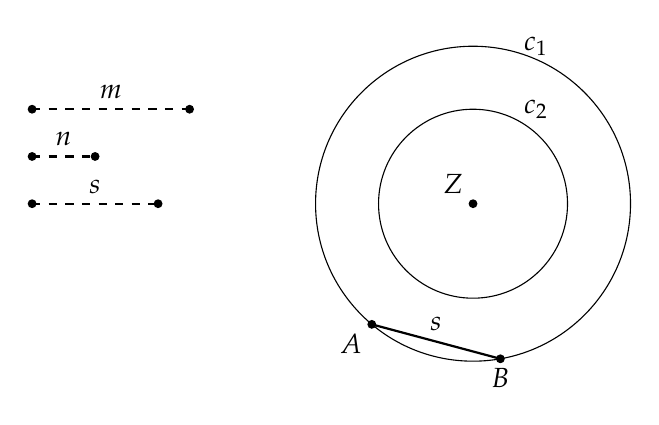
\begin{tikzpicture}[scale=.4]
\coordinate (Z) at (0,0);
\coordinate (A) at (-130:5cm);
\coordinate (B) at (-80:5cm);
\fill (Z) node[above left] {$Z$} circle[radius=4pt];
\fill (A) node[below left] {$A$} circle[radius=4pt];
\fill (B) node[below] {$B$} circle[radius=4pt];
\draw[name path=c1] (Z) circle[radius=5cm];
\draw[name path=c2] (Z) circle[radius=3cm];
\node at (2,5) {$c_1$};
\node at (2,3) {$c_2$};
\draw[thick] (A) -- node[above] {$s$} (B);
\begin{scope}[xshift=-14cm,yshift=3cm]
\coordinate (m) at (0,0);
\coordinate (n) at (0,-1.5);
\coordinate (s) at (0,-3);
\coordinate (mp) at (5,0);
\coordinate (np) at (2,-1.5);
\coordinate (sp) at (4,-3);
\fill (m) circle[radius=4pt];
\fill (n) circle[radius=4pt];
\fill (s) circle[radius=4pt];
\fill (mp) circle[radius=4pt];
\fill (np) circle[radius=4pt];
\fill (sp) circle[radius=4pt];
\draw[thick,dashed] (m) -- node[above] {$m$} (mp);
\draw[thick,dashed] (n) -- node[above] {$n$} (np);
\draw[thick,dashed] (s) -- node[above] {$s$} (sp);
\end{scope}
\end{tikzpicture}
\end{center}

Next lay off any length $w$ from $A$ and $B$ on $c_2$ with $H$ and $K$ on $c_2$ so that $AH = BK = w$:

\begin{center}
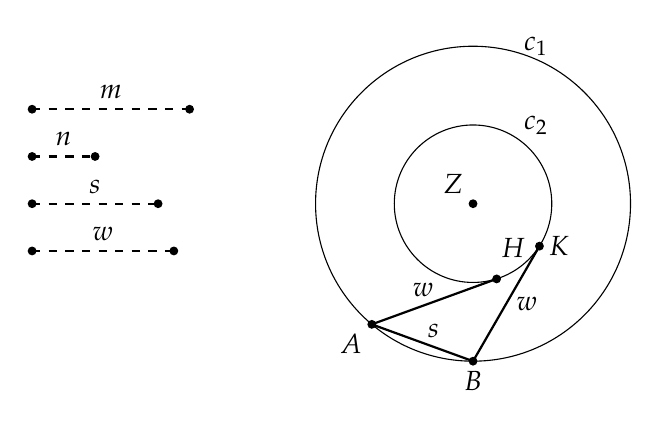
\begin{tikzpicture}[scale=.4]
\coordinate (Z) at (0,0);
\coordinate (A) at (-130:5cm);
\coordinate (B) at (-90:5cm);
\fill (Z) node[above left] {$Z$} circle[radius=4pt];
\fill (A) node[below left] {$A$} circle[radius=4pt];
\fill (B) node[below] {$B$} circle[radius=4pt];
\draw[name path=c1] (Z) circle[radius=5cm];
\draw[name path=c2] (Z) circle[radius=2.5cm];
\node at (2,5) {$c_1$};
\node at (2,2.5) {$c_2$};
\draw[thick] (A) -- node[above,xshift=4pt,yshift=-2pt] {$s$} (B);
\draw[thick] (A) -- node[above,xshift=-4pt,yshift=-2pt] {$w$} +(20:120pt) coordinate (H);
\fill (H) node[above right,xshift=-2pt,yshift=4pt] {$H$} circle[radius=4pt];
\draw[thick] (B) -- node[right] {$w$} +(60:120pt) coordinate (K);
\fill (K) node[right] {$K$} circle[radius=4pt];
\begin{scope}[xshift=-14cm,yshift=3cm]
\coordinate (m) at (0,0);
\coordinate (n) at (0,-1.5);
\coordinate (s) at (0,-3);
\coordinate (w) at (0,-4.5);
\coordinate (mp) at (5,0);
\coordinate (np) at (2,-1.5);
\coordinate (sp) at (4,-3);
\coordinate (wp) at (4.5,-4.5);
\fill (m) circle[radius=4pt];
\fill (n) circle[radius=4pt];
\fill (s) circle[radius=4pt];
\fill (w) circle[radius=4pt];
\fill (mp) circle[radius=4pt];
\fill (np) circle[radius=4pt];
\fill (sp) circle[radius=4pt];
\fill (wp) circle[radius=4pt];
\draw[thick,dashed] (m) -- node[above] {$m$} (mp);
\draw[thick,dashed] (n) -- node[above] {$n$} (np);
\draw[thick,dashed] (s) -- node[above] {$s$} (sp);
\draw[thick,dashed] (w) -- node[above] {$w$} (wp);
\end{scope}
\end{tikzpicture}
\end{center}


$\triangle AHZ$ and $\triangle BKZ$ are congruent by SSS, 

\begin{quote}
The sides are $ZA=ZB=m$ (radius of circle $c_1$), $ZH=ZK=n$ (radius of circle $c_2$, $AH=BK=w$ (by construction).
\end{quote}

\begin{center}
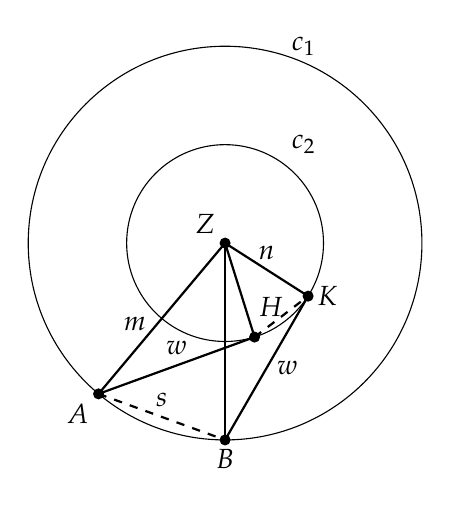
\begin{tikzpicture}[scale=.5]
\coordinate (Z) at (0,0);
\coordinate (A) at (-130:5cm);
\coordinate (B) at (-90:5cm);
\fill (Z) node[above left] {$Z$} circle[radius=4pt];
\fill (A) node[below left] {$A$} circle[radius=4pt];
\fill (B) node[below] {$B$} circle[radius=4pt];
\draw[name path=c1] (Z) circle[radius=5cm];
\draw[name path=c2] (Z) circle[radius=2.5cm];
\node at (2,5) {$c_1$};
\node at (2,2.5) {$c_2$};
\draw[thick,dashed] (A) -- node[above] {$s$} (B);
\draw[thick] (A) -- node[above] {$w$} +(20:120pt) coordinate (H);
\fill (H) node[above right,xshift=-2pt,yshift=4pt] {$H$} circle[radius=4pt];
\draw[thick] (B) -- node[right] {$w$} +(60:120pt) coordinate (K);
\fill (K) node[right] {$K$} circle[radius=4pt];
\draw[thick] (Z) -- node[left,xshift=-2pt,yshift=-2pt] {$m$} (A);
\draw[thick] (Z) -- (B);
\draw[thick] (Z) -- (H);
\draw[thick] (Z) -- node[above] {$n$} (K);
\draw[thick,dashed] (H) -- (K);
\end{tikzpicture}
\end{center}

so $\angle AZH = \angle BZK$ and $\angle AZB = \angle HZK$.

\begin{quote}
This follows by subtraction of angles, but it is somewhat hard to see in the diagram. The following diagram should clarify the construction by displaying only the angles. Since $\alpha_1=\angle AZH = \angle BZK =\alpha_2$ by congruent triangles, we have $\gamma_1 = \alpha_1 - \beta = \alpha_2 - \beta = \gamma_2$.
\begin{center}
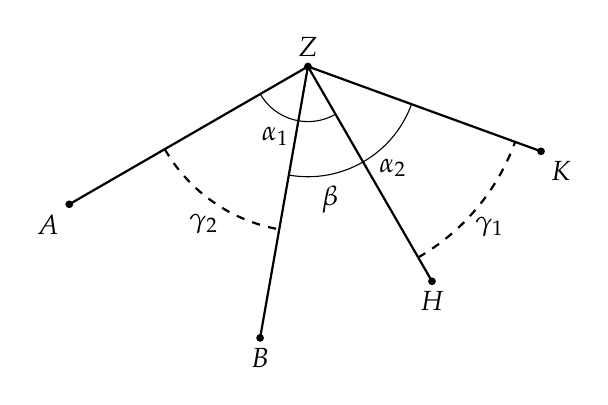
\begin{tikzpicture}[scale=.7]
\coordinate (Z) at (0,0);
\coordinate (A) at (-150:5cm);
\coordinate (B) at (-100:5cm);
\coordinate (H) at (-60:4.5cm);
\coordinate (K) at (-20:4.5cm);
\fill (Z) circle[radius=2pt];
\fill (A) circle[radius=2pt];
\fill (B) circle[radius=2pt];
\fill (H) circle[radius=2pt];
\fill (K) circle[radius=2pt];
\draw[thick] (A) node[below left] {$A$} -- (Z) node[above] {$Z$} -- (B) node[below] {$B$};
\draw[thick] (H) node[below] {$H$} -- (Z) -- (K) node[below right] {$K$};
\draw (-150:1cm) arc (-150:-60:1);
\draw (-100:2cm) arc (-100:-20:2);
\draw[thick,dashed] (-150:3cm) arc (-150:-100:3);
\draw[thick,dashed] (-60:4cm) arc (-60:-20:4);
\node at (-115:1.4) {$\alpha_1$};
\node at (-50:2.4) {$\alpha_2$};
\node[yshift=-3pt] at (-80:2.3) {$\beta$};
\node[yshift=-3pt] at (-40:4.3) {$\gamma_1$};
\node[yshift=-3pt] at (-125:3.3) {$\gamma_2$};
\end{tikzpicture}
\end{center}
\end{quote}

and $\triangle ZAB$ and $\triangle ZHK$ are similar.

\begin{center}
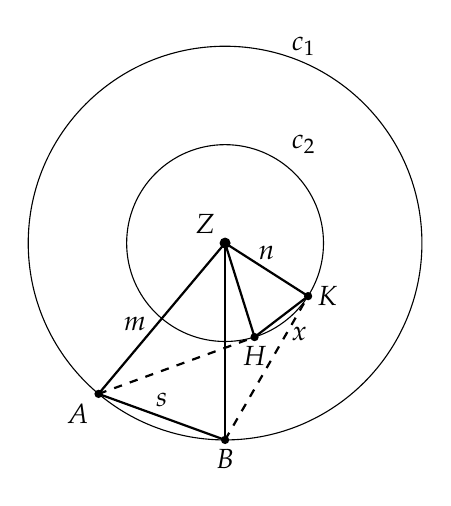
\begin{tikzpicture}[scale=.5]
\coordinate (Z) at (0,0);
\coordinate (A) at (-130:5cm);
\coordinate (B) at (-90:5cm);
\fill (Z) node[above left] {$Z$} circle[radius=4pt];
\fill (A) node[below left] {$A$} circle[radius=3pt];
\fill (B) node[below] {$B$} circle[radius=3pt];
\draw[name path=c1] (Z) circle[radius=5cm];
\draw[name path=c2] (Z) circle[radius=2.5cm];
\node at (2,5) {$c_1$};
\node at (2,2.5) {$c_2$};
\draw[thick] (A) -- node[above] {$s$} (B);
\path[thick,dashed] (A) -- +(20:120pt) coordinate (H);
\fill (H) node[below] {$H$} circle[radius=3pt];
\path[thick,dashed] (B) -- +(60:120pt) coordinate (K);
\fill (K) node[right] {$K$} circle[radius=3pt];
\draw[thick] (Z) -- node[left,xshift=-2pt,yshift=-2pt] {$m$} (A);
\draw[thick] (Z) -- (B);
\draw[thick] (Z) -- (H);
\draw[thick] (Z) -- node[above] {$n$} (K);
\draw[thick] (H) -- node[below right] {$x$} (K);
\draw[thick,dashed] (A) -- (H);
\draw[thick,dashed] (B) -- (K);
\end{tikzpicture}
\end{center}

Then $\frac{m}{s} = \frac{n}{x}$ and $x=\frac{n}{m}s$. \qed

%%%%%%%%%%%%%%%%%%%%%%%%%%%%%%%%%%%%%%%%%%%%%%%%%%%%%%%%%%%%%%%

Now for the solutions to I. and II. above.

\textbf{I’.} Find the point of intersection $S$ of two straight lines $AB$ and $CD$, each of which is given by two points, with compass alone.

\textbf{Solution.} Let $C'$ and $D'$ be reflections of $C$ and $D$ about line $AB$ respectively. The sought-for point of intersection $S$ then lies on line $C'D'$.

\begin{quote}
$CD$ and $C'D'$ intersect $AB$ at the same point $S$ because reflection preserves distance. Given point $S$ defined by the intersection of $AB$ (the line of reflections) and $CD$, $C'S=CS$ and $D'S=DS$.
\end{quote}

\begin{center}
\begin{tikzpicture}[scale=.8]
\coordinate (A) at (-4,0);
\coordinate (B) at (2,0);
\coordinate (C) at (-3,2);
\coordinate (D) at (1,-1);
\coordinate (Cp) at (-3,-2);
\coordinate (Dp) at (1,1);
\fill (A) node[below] {$A$} circle[radius=2pt];
\fill (B) node[below] {$B$} circle[radius=2pt];
\fill (C) node[above] {$C$} circle[radius=2pt];
\fill (D) node[below] {$D$} circle[radius=2pt];
\fill (Cp) node[below] {$C'$} circle[radius=2pt];
\fill (Dp) node[above] {$D'$} circle[radius=2pt];
\draw[name path=ab] ($(A)!1.3!(B)$) -- ($(B)!1.3!(A)$);
\draw[name path=cd] ($(C)!1.2!(D)$) -- node[below,near start] {$e$} ($(D)!1.1!(C)$);
\path [name intersections={of=ab and cd,by={S}}];
\fill (S) node[above] {$S$} circle[radius=2pt];
\draw[thick,dashed] (Cp) -- (Dp);
\draw[thick,dashed] (C) -- node[above left] {$c$} (Cp);
\draw[thick,dashed] (D) -- node[above right] {$d$} (Dp);
\path (C) -- node[right] {$x$} (S);
\node at (-5mm,-2) {\mbox{\boldmath $CD=e$}};
\end{tikzpicture}
\end{center}

$\triangle CSC'$ and $\triangle DSD'$ are similar so $\frac{CS}{DS} = \frac{CC'}{DD'}$. With $x = CS, c = CC', d = DD'$ and $e = CD$, we get $\frac{x}{e-x} = \frac{c}{d}$ or $x=\frac{c}{c+d}e$. (If $D$ is on the same side of $AB$ as $C$, then $x = \frac{c}{c-d}e$.)

\begin{quote}
Here is the diagram corresponding to this situation. The similarity of the triangles $\triangle CSC'$ and $\triangle DSD'$ gives $\frac{x}{x-e}=\frac{c}{d}$ and we can solve for $x=\frac{c}{c-d}e$.
\begin{center}
\begin{tikzpicture}[scale=.8]
\coordinate (A) at (-4,0);
\coordinate (B) at (2,0);
\coordinate (C) at (-3,2);
\coordinate (D) at (-1,1);
\coordinate (Cp) at (-3,-2);
\coordinate (Dp) at (-1,-1);
\fill (A) node[below] {$A$} circle[radius=2pt];
\fill (B) node[below] {$B$} circle[radius=2pt];
\fill (C) node[above] {$C$} circle[radius=2pt];
\fill (D) node[above] {$D$} circle[radius=2pt];
\fill (Cp) node[below] {$C'$} circle[radius=2pt];
\fill (Dp) node[below] {$D'$} circle[radius=2pt];
\draw[name path=ab] ($(A)!1.3!(B)$) -- ($(B)!1.3!(A)$);
\draw[name path=cd] ($(C)!2.2!(D)$) -- node[above, near end] {$e$} ($(D)!1.1!(C)$);
\path [name intersections={of=ab and cd,by={S}}];
\fill (S) node[above] {$S$} circle[radius=2pt];
\draw[thick,dashed] (Cp) -- (S);
\draw[thick,dashed] (C) -- node[above left] {$c$} (Cp);
\draw[thick,dashed] (D) -- node[above right] {$d$} (Dp);
\path (C) -- node[above right,near end] {$x$} (S);
\node at (1,2) {\mbox{\boldmath $CS=x$}};
\end{tikzpicture}
\end{center}
\end{quote}
$c + d = CH$ where $H$ is the intersection point of $c(C',d)$ and $c(D,e)$  on line $CC'$.

\begin{quote}
The proof could simply quote Preliminary problem 3 which claims that given two lengths a line segment whose length is their sum and difference can be computed, but this construction is simpler.

The circle $c(C',d)$ defines the points at distance $d$ from $C'$. We need to construct the intersection of this cricle with the line containing $CC'$. The quadrilateral $C'D'DH$ is a parallelogram since the lengths of both opposite sides are equal. Since $DD'$ is parallel to $CC'$, $C'H$ is also parallel to $DD'$ and therefore on the line containing $CC'$. Since $e$ is the distance $CD$, then $H$, the intersection of $c(D,e)$ with the line containing $CC'$, is also at a distance $e$ from $D$.

\begin{center}
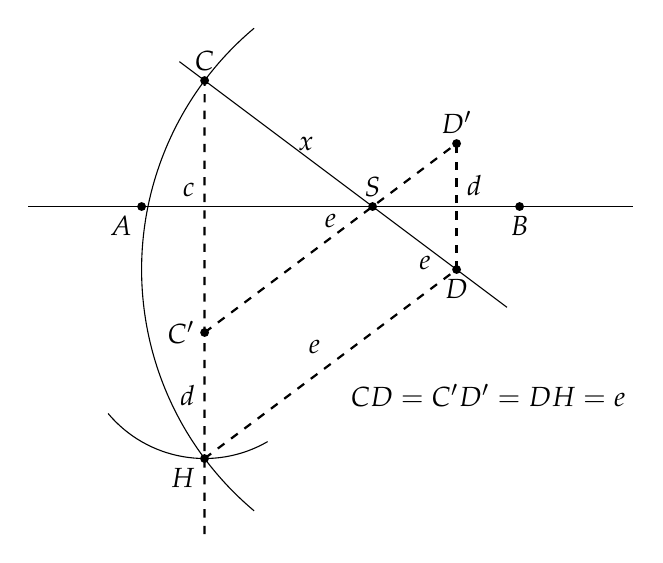
\begin{tikzpicture}[scale=.8]
\coordinate (A) at (-4,0);
\coordinate (B) at (2,0);
\coordinate (C) at (-3,2);
\coordinate (D) at (1,-1);
\coordinate (Cp) at (-3,-2);
\coordinate (Dp) at (1,1);
\fill (A) node[below left] {$A$} circle[radius=2pt];
\fill (B) node[below] {$B$} circle[radius=2pt];
\fill (C) node[above] {$C$} circle[radius=2pt];
\fill (D) node[below] {$D$} circle[radius=2pt];
\fill (Cp) node[left] {$C'$} circle[radius=2pt];
\fill (Dp) node[above] {$D'$} circle[radius=2pt];
\draw[name path=ab] ($(A)!1.3!(B)$) -- ($(B)!1.3!(A)$);
\draw[name path=cd] ($(C)!1.2!(D)$) -- node[below,near start] {$e$} ($(D)!1.1!(C)$);
\path [name intersections={of=ab and cd,by={S}}];
\fill (S) node[above] {$S$} circle[radius=2pt];
\draw[thick,dashed] (Cp) -- node[above] {$e$} (Dp);
\path (C) -- node[above left] {$c$} (Cp);
\draw[thick,dashed] (D) -- node[above right] {$d$} (Dp);
\path (C) -- node[right] {$x$} (S);
\node at (1.5,-3) {$CD=C'D'=DH=e$};
\draw[name path=circled] (D) let
  \p1 = ($ (D) - (C) $),
  \n2 = {veclen(\x1,\y1)}
in
  ++(130:\n2) arc (130:230:\n2);

\draw[name path=circlecp] (Cp) let
  \p1 = ($ (D) - (Dp) $),
  \n2 = {veclen(\x1,\y1)}
in
  ++(-140:\n2) arc (-140:-60:\n2);
\path [name intersections={of=circled and circlecp,by={H}}];
\fill (H) node[below left] {$H$} circle[radius=2pt];
\draw[thick,dashed] ($(C)!1.2!(H)$) -- (C);
\path (H) -- node[left] {$d$} (Cp);
\draw[thick,dashed] (H) -- node[above left] {$e$} (D);
\end{tikzpicture}
\end{center}
\end{quote}

($CH = c - d$ in case $D$ is on the same side of $AB$ as $C$.) Preliminary problem 4 then allows us to construct $x$, and from that $S$ as the intersection of arcs of the circles $c(C,x)$ and $c(C',x)$.

\begin{quote}
$x$ is the length of $CS$ which equals the length of $C'S$ because reflection preserves distances, so all we have to do is compute $x$, and then $S$ will be the intersections of the circles $c(C,x), c(C',x)$. By Preliminary problem 4, we can compute $x=\frac{c}{c+d}e$ given $c,e,d$, where the line segment of length $c+d$ is constructed above as $CH$.
\end{quote}

%%%%%%%%%%%%%%%%%%%%%%%%%%%%%%%%%%%%%%%%%%%%%%%%%%%%%%%%%%%%%%%

\textbf{II’.} Determine the point of intersection $S$ of a given circle $k$ and a given straight line $AB$ with compass alone.

\textbf{Solution.} Let $k = c(M,r)$, and $M'$ be the reflection of $M$ about line $AB$.

\begin{center}
\begin{tikzpicture}[scale=.5]
\coordinate (A) at (-7,0);
\coordinate (B) at (8,0);
\coordinate (M) at (0,-2);
\coordinate (Mp) at (0,2);
\fill (A) node[below] {$A$} circle[radius=3pt];
\fill (B) node[below] {$B$} circle[radius=3pt];
\fill (M) node[below left] {$M$} circle[radius=3pt];
\fill (Mp) node[above left] {$M'$} circle[radius=2pt];
\draw[name path=c1] (M) circle[radius=3cm];
\draw[name path=c2] (Mp) circle[radius=3cm];
\draw[name path=ab] ($(A)!1.2!(B)$) -- ($(B)!1.2!(A)$);
\path [name intersections={of=c1 and c2,by={S1,S2}}];
\fill (S1) circle[radius=3pt];
\fill (S2) circle[radius=3pt];
\path[name path=radius1] (M) -- ++(15:4cm);
\path [name intersections={of=c1 and radius1,by={R1}}];
\draw[thick,dashed] (M) -- node[below] {$r$} (R1);
\path[name path=radius2] (Mp) -- ++(40:4cm);
\path [name intersections={of=c2 and radius2,by={R2}}];
\draw[thick,dashed] (Mp) -- node[above] {$r$} (R2);
\fill (R1) circle[radius=3pt];
\fill (R2) circle[radius=3pt];
\end{tikzpicture}
\end{center}

The points of intersection are the points where $c(M,r)$ and $c(M',r)$ intersect. This construction cannot be done if $M$ is on line $AB$.

\begin{center}
\begin{tikzpicture}[scale=.5]
\coordinate (A) at (-7,0);
\coordinate (B) at (8,0);
\coordinate (M) at (0,0);
\fill (A) node[below] {$A$} circle[radius=3pt];
\fill (B) node[below] {$B$} circle[radius=3pt];
\fill (M) node[below left] {$M$} circle[radius=3pt];
\draw[name path=c1] (M) circle[radius=3cm];
\draw[name path=ab] ($(A)!1.2!(B)$) -- ($(B)!1.2!(A)$);
\path[name path=radius1] (M) -- ++(-30:4cm);
\path [name intersections={of=c1 and radius1,by={R1}}];
\draw[thick,dashed] (M) -- node[below] {$r$} (R1);
\path [name intersections={of=c1 and ab,by={S1,S2}}];
\fill (S1) node[above right] {$AM+r$} circle[radius=3pt];
\fill (S2) node[above left] {$AM-r$} circle[radius=3pt];
\fill (R1) circle[radius=3pt];
\end{tikzpicture}
\end{center}
In this exceptional case, extend and shorten $AM$ by $r$ by Prelim 3; the end points of the extended and shortended sements are the desired points. \qed

\end{document}

